Город Мехико расположен в прекрасной долине, известной как Долина Мехико, на месте
которой много лет назад было озеро. Около 1300 года ацтекские религиозные лидеры
выпустили указ о том, что центр озера должен быть засыпан, чтобы построить столицу их
империи. В настоящее время озеро полностью осушено.

Вокруг озера до появления ацтеков были расположены c прибрежных городов. Некоторые из
этих городов заключили между собой коммерческие соглашения. Между городами,
установившими коммерческие соглашения, по озеру на лодках перевозились различные
товары. Любую пару городов можно было соединить отрезком прямой, полностью
проходящим через озеро.

В какой-то момент короли городов решили упорядочить товароперевозки. Они разработали
маршрут товароперевозок, который соединяет все города вокруг озера. Маршрут
удовлетворяет следующим условиям:
\begin{itemize}
\item Он начинается в каком-либо городе, проходит через каждый прибрежный город и
заканчивается в городе, отличном от того, в котором он начался.
\item Маршрут проходит через каждый город ровно один раз.
\item Любые два последовательно посещаемых города маршрута обязаны иметь между
собой коммерческое соглашение.
\item Маршрут состоит из отрезков прямых, каждый из которых соединяет два
последовательно посещаемых города маршрута.
\item Чтобы избежать столкновения лодок, маршрут не должен иметь самопересечений.
\end{itemize}

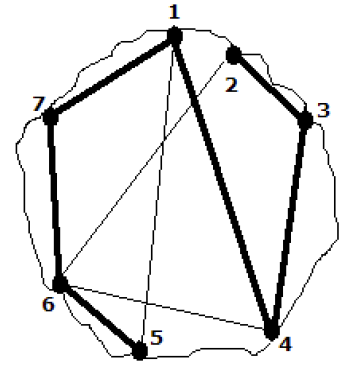
\includegraphics{mexico.png}

На рисунке показано озеро и города вокруг него. Тонкие и жирные линии отрезков обозначают коммерческие соглашения между городами. Жирные линии показывают маршрут грузоперевозок, начинающийся в городе 2 и заканчивающийся в городе 5.

Этот маршрут нигде не имеет самопересечений. Но если построить маршрут, идущий из города 2 в город 6, затем в город 5, а затем в город 1, то он будет
неправильным, поскольку имеет самопересечения. 

Города нумеруются целыми числами от 1 до $c$ по направлению часовой стрелки. 

Напишите программу, которая по заданному числу городов $c$ и списку коммерческих
соглашений между городами, найдет маршрут товароперевозок, удовлетворяющий
указанным выше условиям